\documentclass{article}
\usepackage[left=8em,right=8em]{geometry}
\usepackage{amsmath,amsthm,amssymb}
\usepackage{lineno}
\usepackage{relsize}
\usepackage{graphicx}
%\linenumbers
\renewcommand*{\proofname}{Proof}
\date{}
\author{}
\begin{document}
\centerline{\textbf{Exercises for Section 11.1}}
$ $\newline
\textbf{Ex 1.} The set $R= \{(5,0),(5,1),(5,2),(5,3),(5,4),(4,0),(4,1),(4,2),(4,3),(3,0),(3,1), (3,2),(2,0),(2,1),(1,0) \}$ is the $>$ relation on $A$. Diagram of $R$:
\begin{figure}[h]
\centering
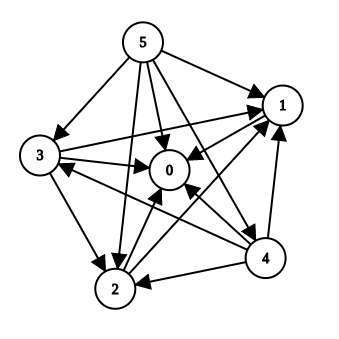
\includegraphics[scale=0.5]{1.png}
\end{figure}\\
\textbf{Ex 2.} The set $R= \{(1,1), (1,2), (1,3), (1,4), (1,5), (1,6), (2,2), (2,4), (2,6), (3,3), (3,6), (4,4), (5,5), (6,6) \}$ is the $|$ (divides) relation on $A$. Diagram of $R$:
\begin{figure}[h]
\centering
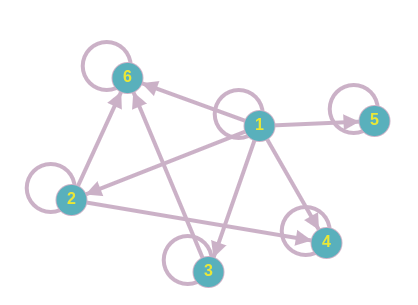
\includegraphics[scale=0.6]{2.png}
\end{figure}\\
\newpage
\noindent \textbf{Ex 3.} The set $R= \{(0,0), (1, 0), (1, 1), (2, 0), (2,1), (2,2), (3,0), (3,1), (3,2), (3,3), (4, 0), (4,1), (4,2), (4,3), (4,4),\\ (5, 0), (5,1), (5,2), (5,3), (5,4), (5,5) \}$ is the $\geq$ relation on $A$. Diagram of $R$:
\begin{figure}[h]
\centering
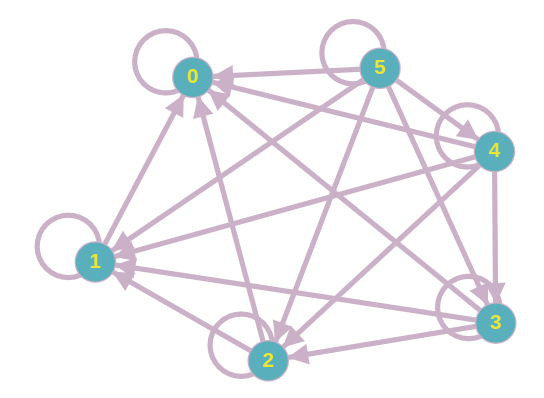
\includegraphics[scale=0.5]{3.png}
\end{figure}\\
\textbf{Ex 4.}\\
$A=\{0,1,2,3,4,5\}$ and $R=\{(0,0), (0,4), (1,1),(1,3),(1,5),(2,2),(2,4),(3,3),(3,1),(4,4),(4,0),(4,2),(5,5),(5,1)\}$.\\
$ $\newline
\textbf{Ex 5.}
$A=\{0,1,2,3,4,5\}$ and $R=\{(1,2), (2,5), (3,3), (4,2), (4,3),(5,0)\}$.\\
$ $\newline
\textbf{Ex 6.}
$R=\{ (x,y) \in \mathbb{Z} \times \mathbb{Z}: x \equiv y \pmod{5} \}$.\\
$ $\newline
\textbf{Ex 7.}
$R=\{ (x,y) \in \mathbb{Z} \times \mathbb{Z}: y-x \in \mathbb{N} \}$.\\
$ $\newline
\textbf{Ex 8.}
Diagram of R:
\begin{figure}[h]
\centering
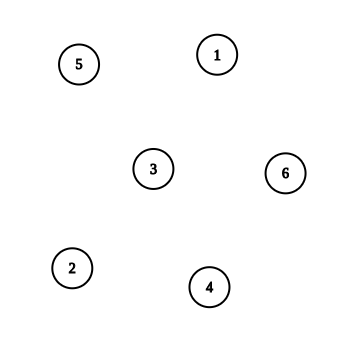
\includegraphics[scale=0.5]{4.png}
\end{figure}
\newpage
\noindent \textbf{Ex 9.} The number of relations on $A$ is equivalent to the number of subsets of $A \times A$. Because $|A|=6$, it follows that $|A \times A|=|A|\cdot{}|A|=6^2=36$. The number of subsets of a set with $36$ elements is then $2^{36}$. Thus there are $2^{36}$ different relations on $A$.\\
$ $\newline
\noindent \textbf{Ex 10.} The set $\{ (x,x) : x \in \mathbb{R} \}$ is the equality relation on $\mathbb{R}$. When we subtract that from cartesian product of $\mathbb{R}$ with itself we get the inequality relation on $\mathbb{R}$.\\
$ $\newline
\noindent \textbf{Ex 11.} There are $2^{|A^2|}$ different relations on A.\\
$ $\newline
\noindent \textbf{Ex 12.} $R$ is the $\geq$ relation on $\mathbb{R}$.

$ $\newline
\noindent \textbf{Ex 13.} $R$ is the inequality relation on $\mathbb{R}$.\\
$ $\newline
\noindent \textbf{Ex 14.} $R$ is the $<$ relation on $\mathbb{Z}$.\\
$ $\newline
\noindent \textbf{Ex 15.} $R = \{(x,y) \in \mathbb{Z} : 3|abs(x-y)\}$.
\end{document}

